\documentclass[usenames,dvipsnames]{beamer}

%& PACKAGES
\usepackage{graphicx}
\usepackage{amsmath,amsfonts,amssymb,amsthm}
\usepackage{mathtools}
\usepackage[noend]{algorithmic}
\usepackage{algorithm}
\usepackage{environ}
\usepackage{xcolor}
\usepackage{caption}
\usepackage{multicol}
\usepackage{array}
\usepackage[algo2e,vlined,ruled]{algorithm2e}
\usepackage{hyperref}
\usepackage{tcolorbox}
\usepackage{wasysym}
\usepackage{transparent}
\usepackage{relsize}
\usepackage{appendixnumberbeamer}
\usepackage[export]{adjustbox}
\usepackage{wrapfig}
\usepackage[absolute,overlay]{textpos}
\usepackage[utf8]{inputenc}
%\usepackage[texcoord, grid, gridcolor=red!10, subgridcolor=green!10, gridunit=cm]{eso-pic}
\usepackage{tikzit}
\usepackage{adjustbox}
\usepackage{pgfgantt}
\usepackage{tikz}
\usepackage{pgfplots}
\usetikzlibrary{shapes,fit,arrows,backgrounds,positioning,fadings,shadows,intersections, pgfplots.fillbetween,shapes.misc,automata,patterns}

\tikzset{
	cross/.style={
		cross out,
		draw=black,
		minimum size=2*(#1-\pgflinewidth),
		inner sep=0mm,
		outer sep=0mm
	},
	cross/.default={1mm} % default radius
}

\hypersetup{
	colorlinks=false,
	urlcolor=cyan,
	citecolor=black
}

%& BEAMER SETTINGS
\usetheme{default}
% \usecolortheme{seagull}

\setbeamertemplate{blocks}[rounded]% Rounded blocks

\useoutertheme[subsection=false]{miniframes}

\makeatletter
\let\beamer@writeslidentry@miniframeson=\beamer@writeslidentry
\def\beamer@writeslidentry@miniframesoff{%
  \expandafter\beamer@ifempty\expandafter{\beamer@framestartpage}{}% does not happen normally
  {%else
    % removed \addtocontents commands
    \clearpage\beamer@notesactions%
  }
}
\newcommand*{\miniframeson}{\let\beamer@writeslidentry=\beamer@writeslidentry@miniframeson}
\newcommand*{\miniframesoff}{\let\beamer@writeslidentry=\beamer@writeslidentry@miniframesoff}
\makeatother

\setbeamerfont{footnote}{size=\tiny}
\setbeamerfont{frametitle}{size=\large}


\title{PhD Title}
\author{Franco Peschiera}
\date{}

\setbeamerfont{frametitle}{size=\large}

\begin{document}
{
	\setbeamertemplate{footline}{} 
	\begin{frame}{}%
		\begin{picture}(0,0)%
			%\makebox(600,-40)[]{
\includegraphics[width=2cm]{images/logos/universite}}
		\end{picture}
		\vspace{1cm}
		\titlepage
		\vspace{-1cm}
		\begin{figure}%
			\centering
			%\makebox[\textwidth][c]{\includegraphics[width=1.1\textwidth]{images/logos/all-logos}}%
		\end{figure}%
	\end{frame}
}
\addtocounter{framenumber}{-1}

\def\introtitle{Introduction}
\def\oltatitle{Le compromis planification \vs{} re-planification}
\def\ratstitle{Planifier dans un MDP évoluant graduellement avec le temps}
\def\llrltitle{Apprendre dans un MDP évoluant brusquement avec le temps}
\def\conclusiontitle{Conclusion générale}

\def\sommvspace{2em}

\begin{frame}
\tableofcontents[hideallsubsections]
\end{frame}
\begin{frame}

\begin{block}{Contents}

\begin{enumerate}[<+->]

\item \introtitle
\item
  Complexity and exact methods.
\item
  Second contribution.
\item
  Third contribution.
\item
  Conclusions.
\end{enumerate}

\end{block}

\end{frame}

\begin{frame}

\end{frame}

\hypertarget{introduction}{%
\section{Introduction}\label{introduction}}

\begin{itemize}[<+->]
\item
  Maintenance planning is more important.
\item
  Complexity and durability are growing with time.

  \begin{itemize}[<+->]
  
  \item
    buildings that need to last 100 years.
  \item
    green energy needs lasting infrastructure.
  \end{itemize}
\end{itemize}

\begin{frame}{The maintenance planning problem}
\protect\hypertarget{the-maintenance-planning-problem}{}

Three main concepts in all maintenance planning:

\begin{itemize}[<+->]

\item
  Resources.
\item
  Tasks.
\item
  Recovery tasks.
\end{itemize}

\emph{time}

Examples: industrial production, nurse rostering, aircraft.

\end{frame}

\begin{frame}{An MFMP problem}
\protect\hypertarget{an-mfmp-problem}{}

\begin{itemize}[<+->]

\item
  Aircraft.
\item
  Missions.
\item
  Maintenances.
\end{itemize}

Objective:

\end{frame}

\begin{frame}

\begin{block}{An MFMP solution}

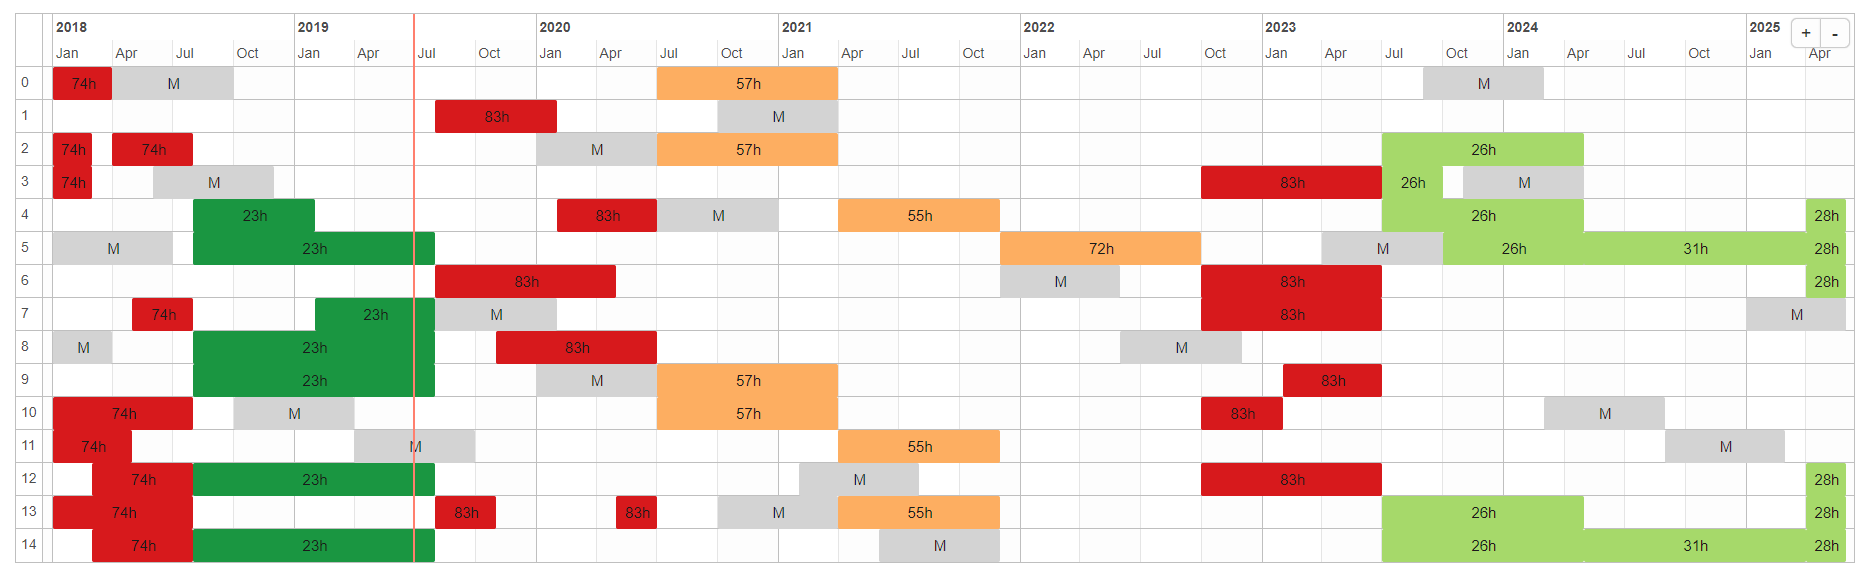
\includegraphics[width=0.7\linewidth]{calendar3}

\end{block}

\end{frame}

\begin{frame}

\begin{block}{Encoding of an MFMP solution}

\begin{align}
 a_{it} = 
  \begin{cases} 
   -1 & check \\
   0 & no\,\,assignment \\
   j & mission\,\, j \\
  \end{cases}\notag
\end{align}

Table format: a solution \(x\) is represented by a matrix
\(A = \mathbb{Z}^{I \times T}\).

Patterns: \(p \in \mathcal{P}\)

\(p = \{a_{i0}, a_{it}, a_{it+1}, ..., a_{iT}\}\)

Pattern format: a solution \(x\) is represented by a mapping
\(f: \mathcal{I} \to \mathcal{P}\).

\end{block}

\end{frame}

\begin{frame}

\begin{block}{Contents}

\begin{enumerate}[<+->]

\item
  Introduction.
\item
  Complexity analysis and exact methods.
\item
  Pattern-like modeling and machine learning.
\item
  Efficient pattern-generation with DP.
\end{enumerate}

\end{block}

\end{frame}

\begin{frame}

\begin{block}{Complexity analysis}

safdasdf

\end{block}

\end{frame}

\begin{frame}

\begin{block}{Exact methods}

\begin{tabular}{p{15mm}p{110mm}}
  $a_{jit}$ &  :  =1 if mission $j \in J$ in period $t \in \mathcal{T}_j$ is realized with aircraft $i \in \mathcal{I}_j$, 0 otherwise.  \\
  $m_{it}$   & :  =1 if aircraft $i \in I$ starts a check in period $t \in \mathcal{T}$, 0 otherwise.  \\
  $u_{it}$    &:  flown time (continuous) by aircraft $i \in I$ during period $t \in \mathcal{T}$. \\
\end{tabular}

\begin{align}
 & u_{it} \geq \sum_{j \in \mathcal{J}_t \cap \mathcal{O}_i} a_{jti} H_j 
    & t =1, ..., \mathcal{T}, i \in \mathcal{I} \label{eq:flight1}\\
 & u_{it} \geq U^{min} (1 - \sum_{t' \in \mathcal{T}^s_t} m_{it'})
    & t =1, ..., \mathcal{T}, i \in \mathcal{I} \label{eq:flight2}\\
 & rft_{it} \leq rft_{i(t-1)} - u_{it} + H^M m_{it}
    & t =1, ..., \mathcal{T}, i \in \mathcal{I} \label{eq:first_rft_upper}\\
& rft_{it} \in [0,H^M]
      & t \in \mathcal{T}, i \in \mathcal{I} \label{eq:first-mu}
\end{align}

\end{block}

\begin{block}{Contents}

\begin{enumerate}[<+->]

\item
  Introduction.
\item
  Complexity analysis and exact methods.
\item
  Pattern-like modeling and machine learning.
\item
  Efficient pattern-generation with DP.
\end{enumerate}

\end{block}

\end{frame}

\begin{frame}

\begin{block}{New formulation}

\begin{tabular}{p{15mm}p{110mm}}
  $a_{ijtt'}$ & : =1 if aircraft $i$ starts an assignment to mission $j$ at the beginning of period $t$ and finishes at the end of period $t'$, zero otherwise.  \\
  $m_{ip}$ &: =1 if aircraft $i$ uses check pattern $p$, zero otherwise.
 each pattern $p$ has a single feasible combination of check starts for an aircraft during the whole planning (usually only 1-2 checks per aircraft). \\
\end{tabular}

\begin{align}
  & \sum_{(j, t, t') \in \mathcal{J}\mathcal{T}\mathcal{T}_{ic}} a_{ijtt'} H^\prime_{jtt'} + U^{\prime}_{tc} \leq H^{M} + M (1 - m_{ip}) & \notag \\
  & \hspace{200px}  i \in \mathcal{I}, p \in \mathcal{P}, c \in \mathcal{C}_p \label{eq:cycle_hours2}\\
\end{align}

\end{block}

\end{frame}

\begin{frame}

\begin{block}{Formulation}

\begin{align}
  & \text{Max}\;
  \sum_{i \in \mathcal{I}, p \in \mathcal{P}} m_{ip} \times W_p \\
  & \sum_{i \in \mathcal{I}, p \in \mathcal{P}_{t}} m_{ip} \leq C^{max} 
          & t \in \mathcal{T} \label{eq:capacity1}\\
  & \sum_{i \in \mathcal{I}_j, (t_1, t_2) \in \mathcal{T}_{jt}} a_{ijt_1t_2} \geq R_j
          & j \in \mathcal{J}, t \in \mathcal{TJ}_j  \label{eq:missionres}\\
  & \sum_{p \in \mathcal{P}_{t}} m_{ip} + \sum_{j \in \mathcal{J}_t \cap \mathcal{J}_i} \sum_{(t_1, t_2) \in \mathcal{T}_{jt}} a_{ijt_1t_2} \leq 1 
          & t \in \mathcal{T}, i \in \mathcal{I} \label{eq:state}\\
  & \sum_{(j, t, t') \in \mathcal{J}\mathcal{T}\mathcal{T}_{ic}} a_{ijtt'} H^\prime_{jtt'} + U^{\prime}_{tc} \leq H^M + M (1 - m_{ip}) & \notag \\
    & & i \in \mathcal{I}, p \in \mathcal{P}, c \in \mathcal{C}_p \\
\end{align}

\end{block}

\end{frame}

\begin{frame}

\begin{block}{New vs old formulation}

\begin{enumerate}[<+->]

\item
  It uses 3 times the number of constraints and 3 times the number of
  variables.
\end{enumerate}

\begin{itemize}[<+->]

\item
  variables: 11000 =\textgreater{} 28000.
\item
  constraints: 13000 =\textgreater{} 48000.
\end{itemize}

\begin{enumerate}[<+->]

\item
  It is still better. Better lineal relaxation, better performance.
\item
  Can we reduce intelligently the number of variables?
\end{enumerate}

\begin{itemize}[<+->]

\item
  we can.
\end{itemize}

\end{block}

\end{frame}

\begin{frame}

\begin{block}{Predicting pseudo-cuts}

Let an optimization problem with input data \(x\) and solution space
\(y \in \mathcal{Y}(x)\). We want to find the optimal solution given a
cost function \(C(x,y)\):

\[
y^{*}(x) :\equiv arg \,\,\min_{y \in \mathcal{Y}(x)} C(x,y)
\]

For any solution \(y\), we can calculate \(N\) several features
\(g_n(y) \,\, \forall n \in \{1, .., N\}\).

\[
\hat{g}_n(x) \approx g_n(y^{*}) \,\, \forall n \in \{1, .., N\}
\]

We then use that information to reduce the solution space
\(\mathcal{Y}^\prime(x) \subset \mathcal{Y}(x)\) and solve it:

\[\hat{y}^{*}(x) = arg \,\,\min_{y \in \mathcal{Y}^\prime(x)} C(x,y)\]

The trick is doing so without losing optimality:

\begin{align}
    C(x,\hat{y}^{*}(x)) \approx  C(x,y^{*}(x) ) \notag
\end{align}

\end{block}

\end{frame}

\begin{frame}

\begin{block}{Distance between maintenances}

.pull-left{[} * The distance between maintenance has a maximum of
\(E^{M}\) periods. * Depending on the instance, the optimal distance can
be shorter. * This distance conditions the total number of patterns to
create.{]}

.pull-right{[}

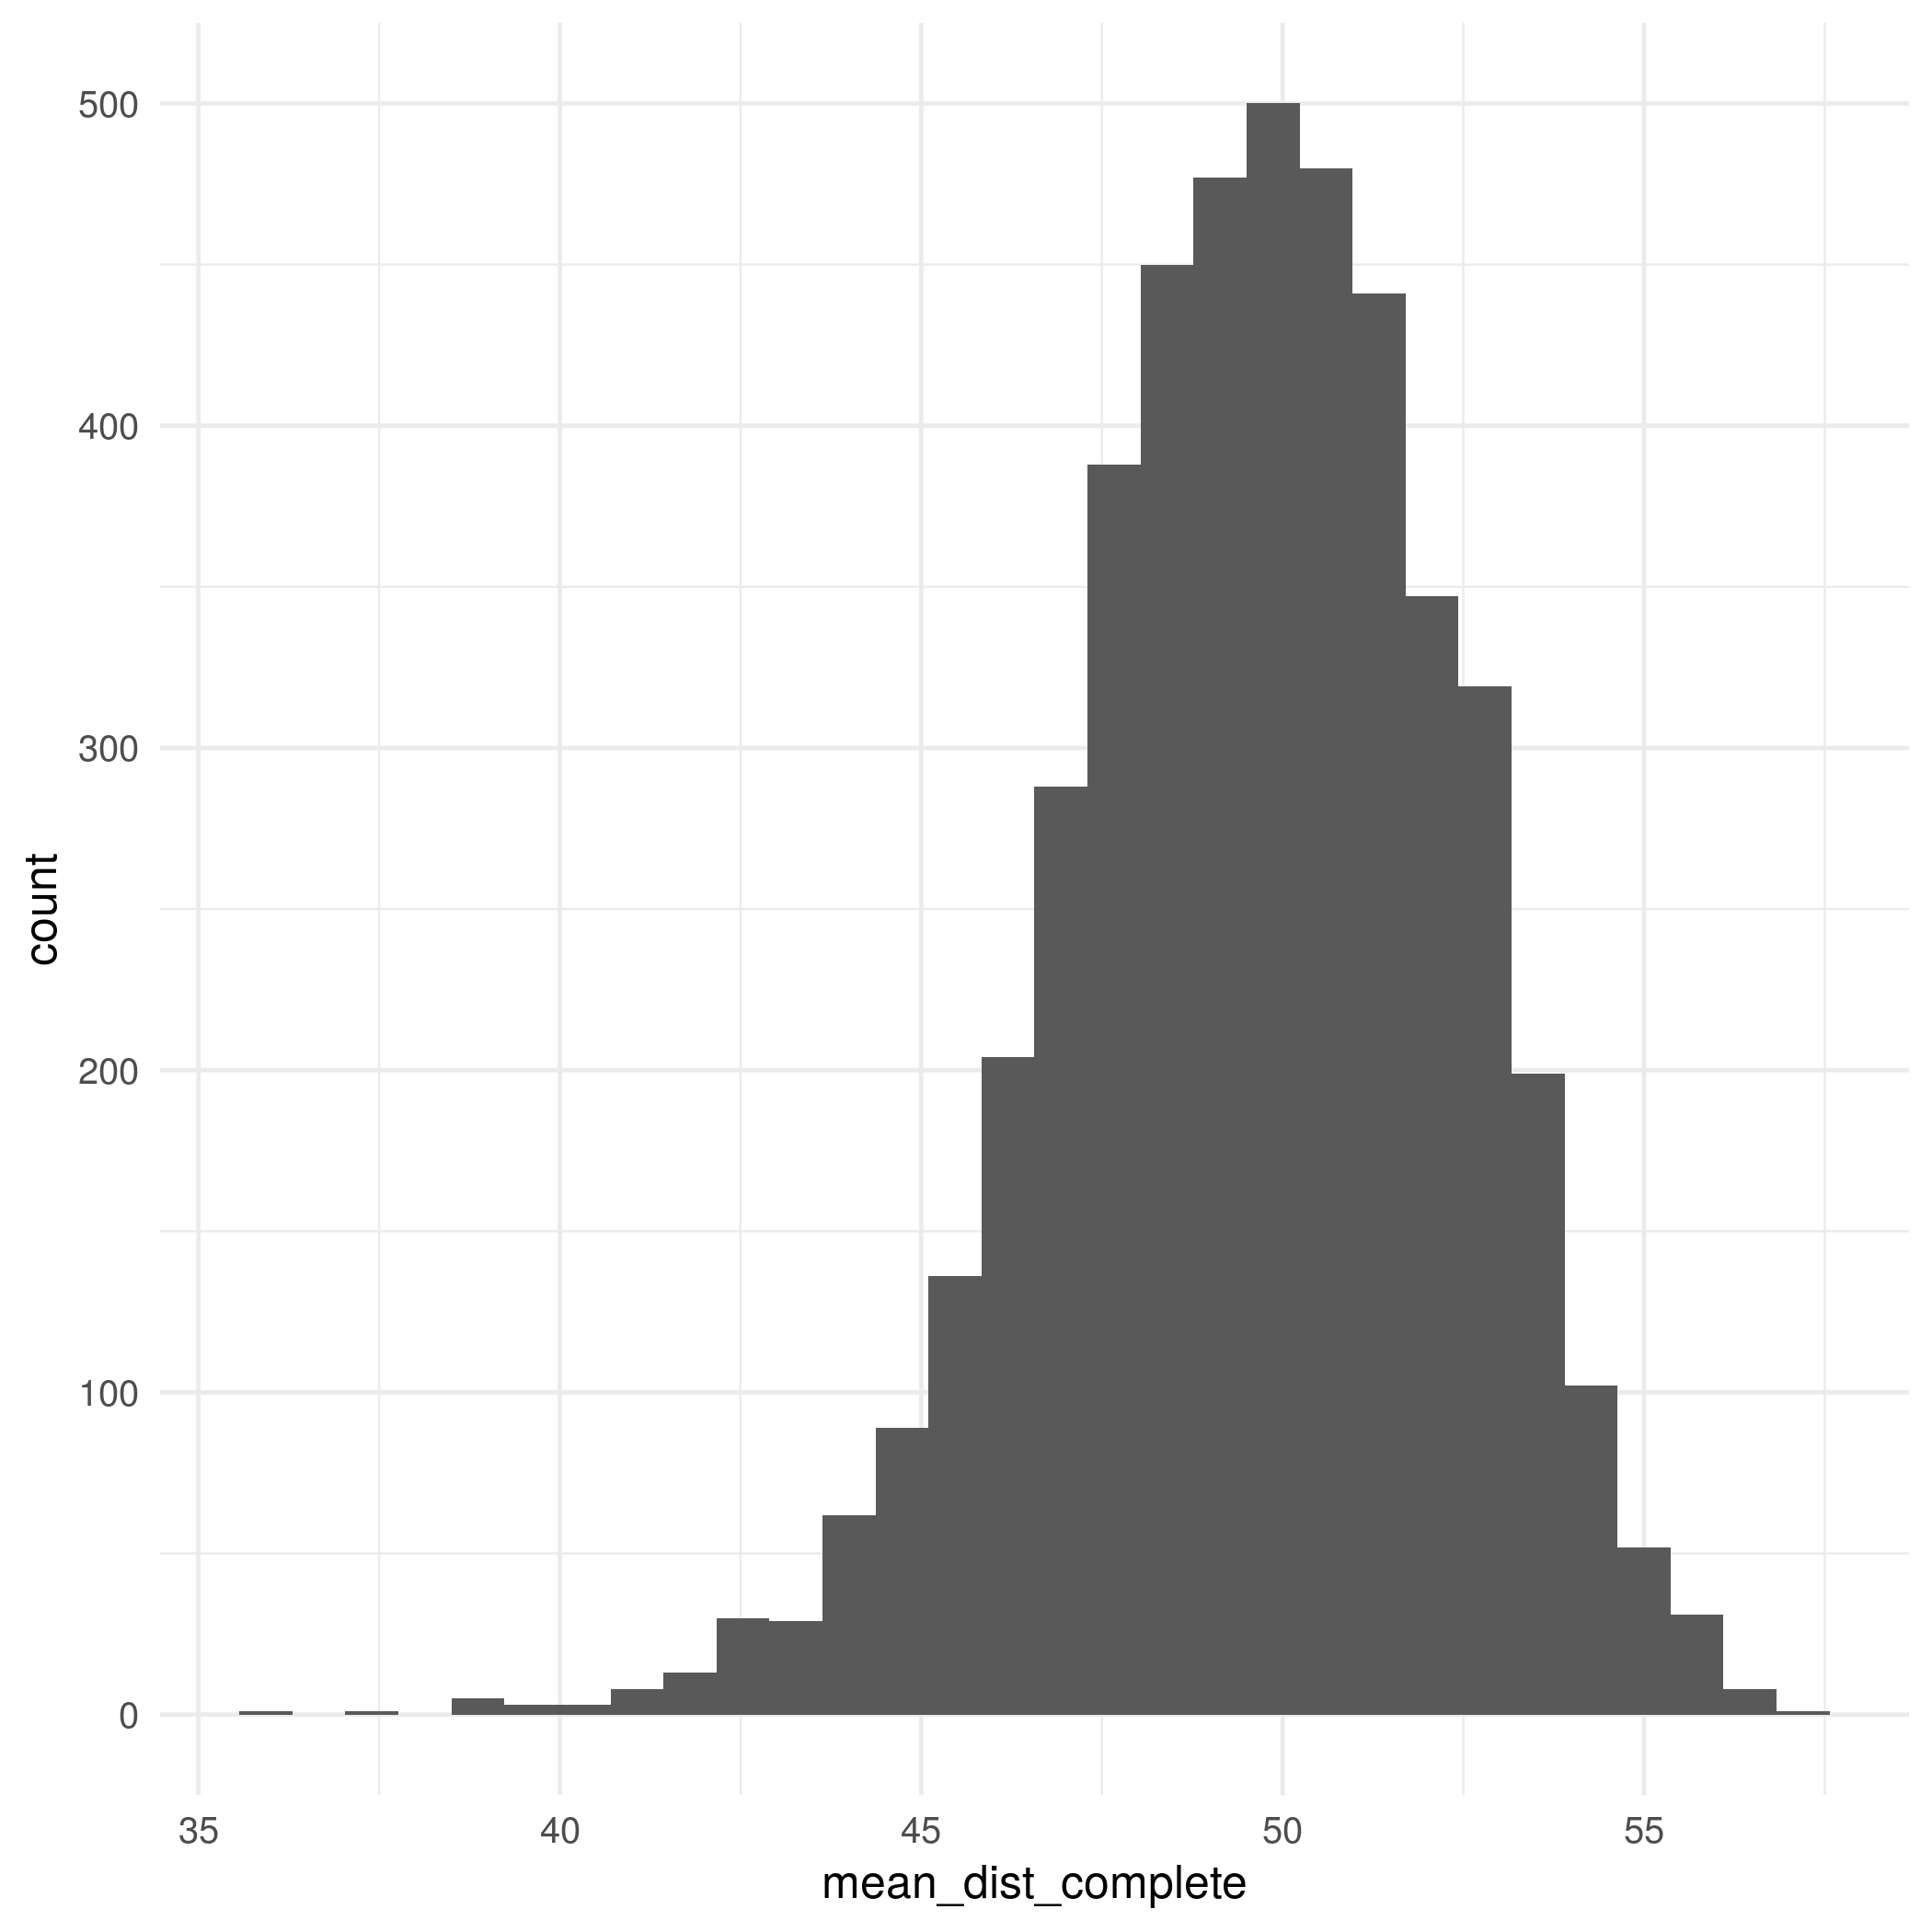
\includegraphics[width=1\linewidth]{hist_mean_dist_complete_IT000125_20190716}
{]}

\end{block}

\end{frame}

\begin{frame}

\begin{block}{Forecasting + Optimization}

\textbf{We want to}:

\begin{enumerate}[<+->]

\item
  Train a statistical model to predict the mean distance between
  maintenances for any given instance.
\item
  Use this information to limit all possible combinations of patterns to
  generate.
\end{enumerate}

--

\textbf{Benefits}:

\begin{enumerate}[<+->]

\item
  \textbf{Performance}: a smaller model is easier to solve.
\item
  \textbf{User feedback}: direct feedback about the solution without
  needing to solve any model.
\item
  \textbf{More stable solutions}: Every aircraft flies an amount that is
  closest to the mean of the fleet.
\end{enumerate}

--

\textbf{The better we're able to predict the optimal distance between
maintenances for the whole fleet, the less optimality we will lose}

\end{block}

\end{frame}

\begin{frame}

\begin{block}{Prediction model}

.pull-left{[} * \textbf{Technique}: \emph{Quantile regressions} to
estimate upper and lower bounds. * \textbf{Training}: 5000 small
instances. * \textbf{Input features}: * mean flight demand per period, *
total remaining flight hours at start (init), * variance of flight
demand, * demand of special missions, * number of period where flight
demand is cut in two. * \textbf{Output features}: mean distance between
maintenances.{]}

--

.pull-right{[}

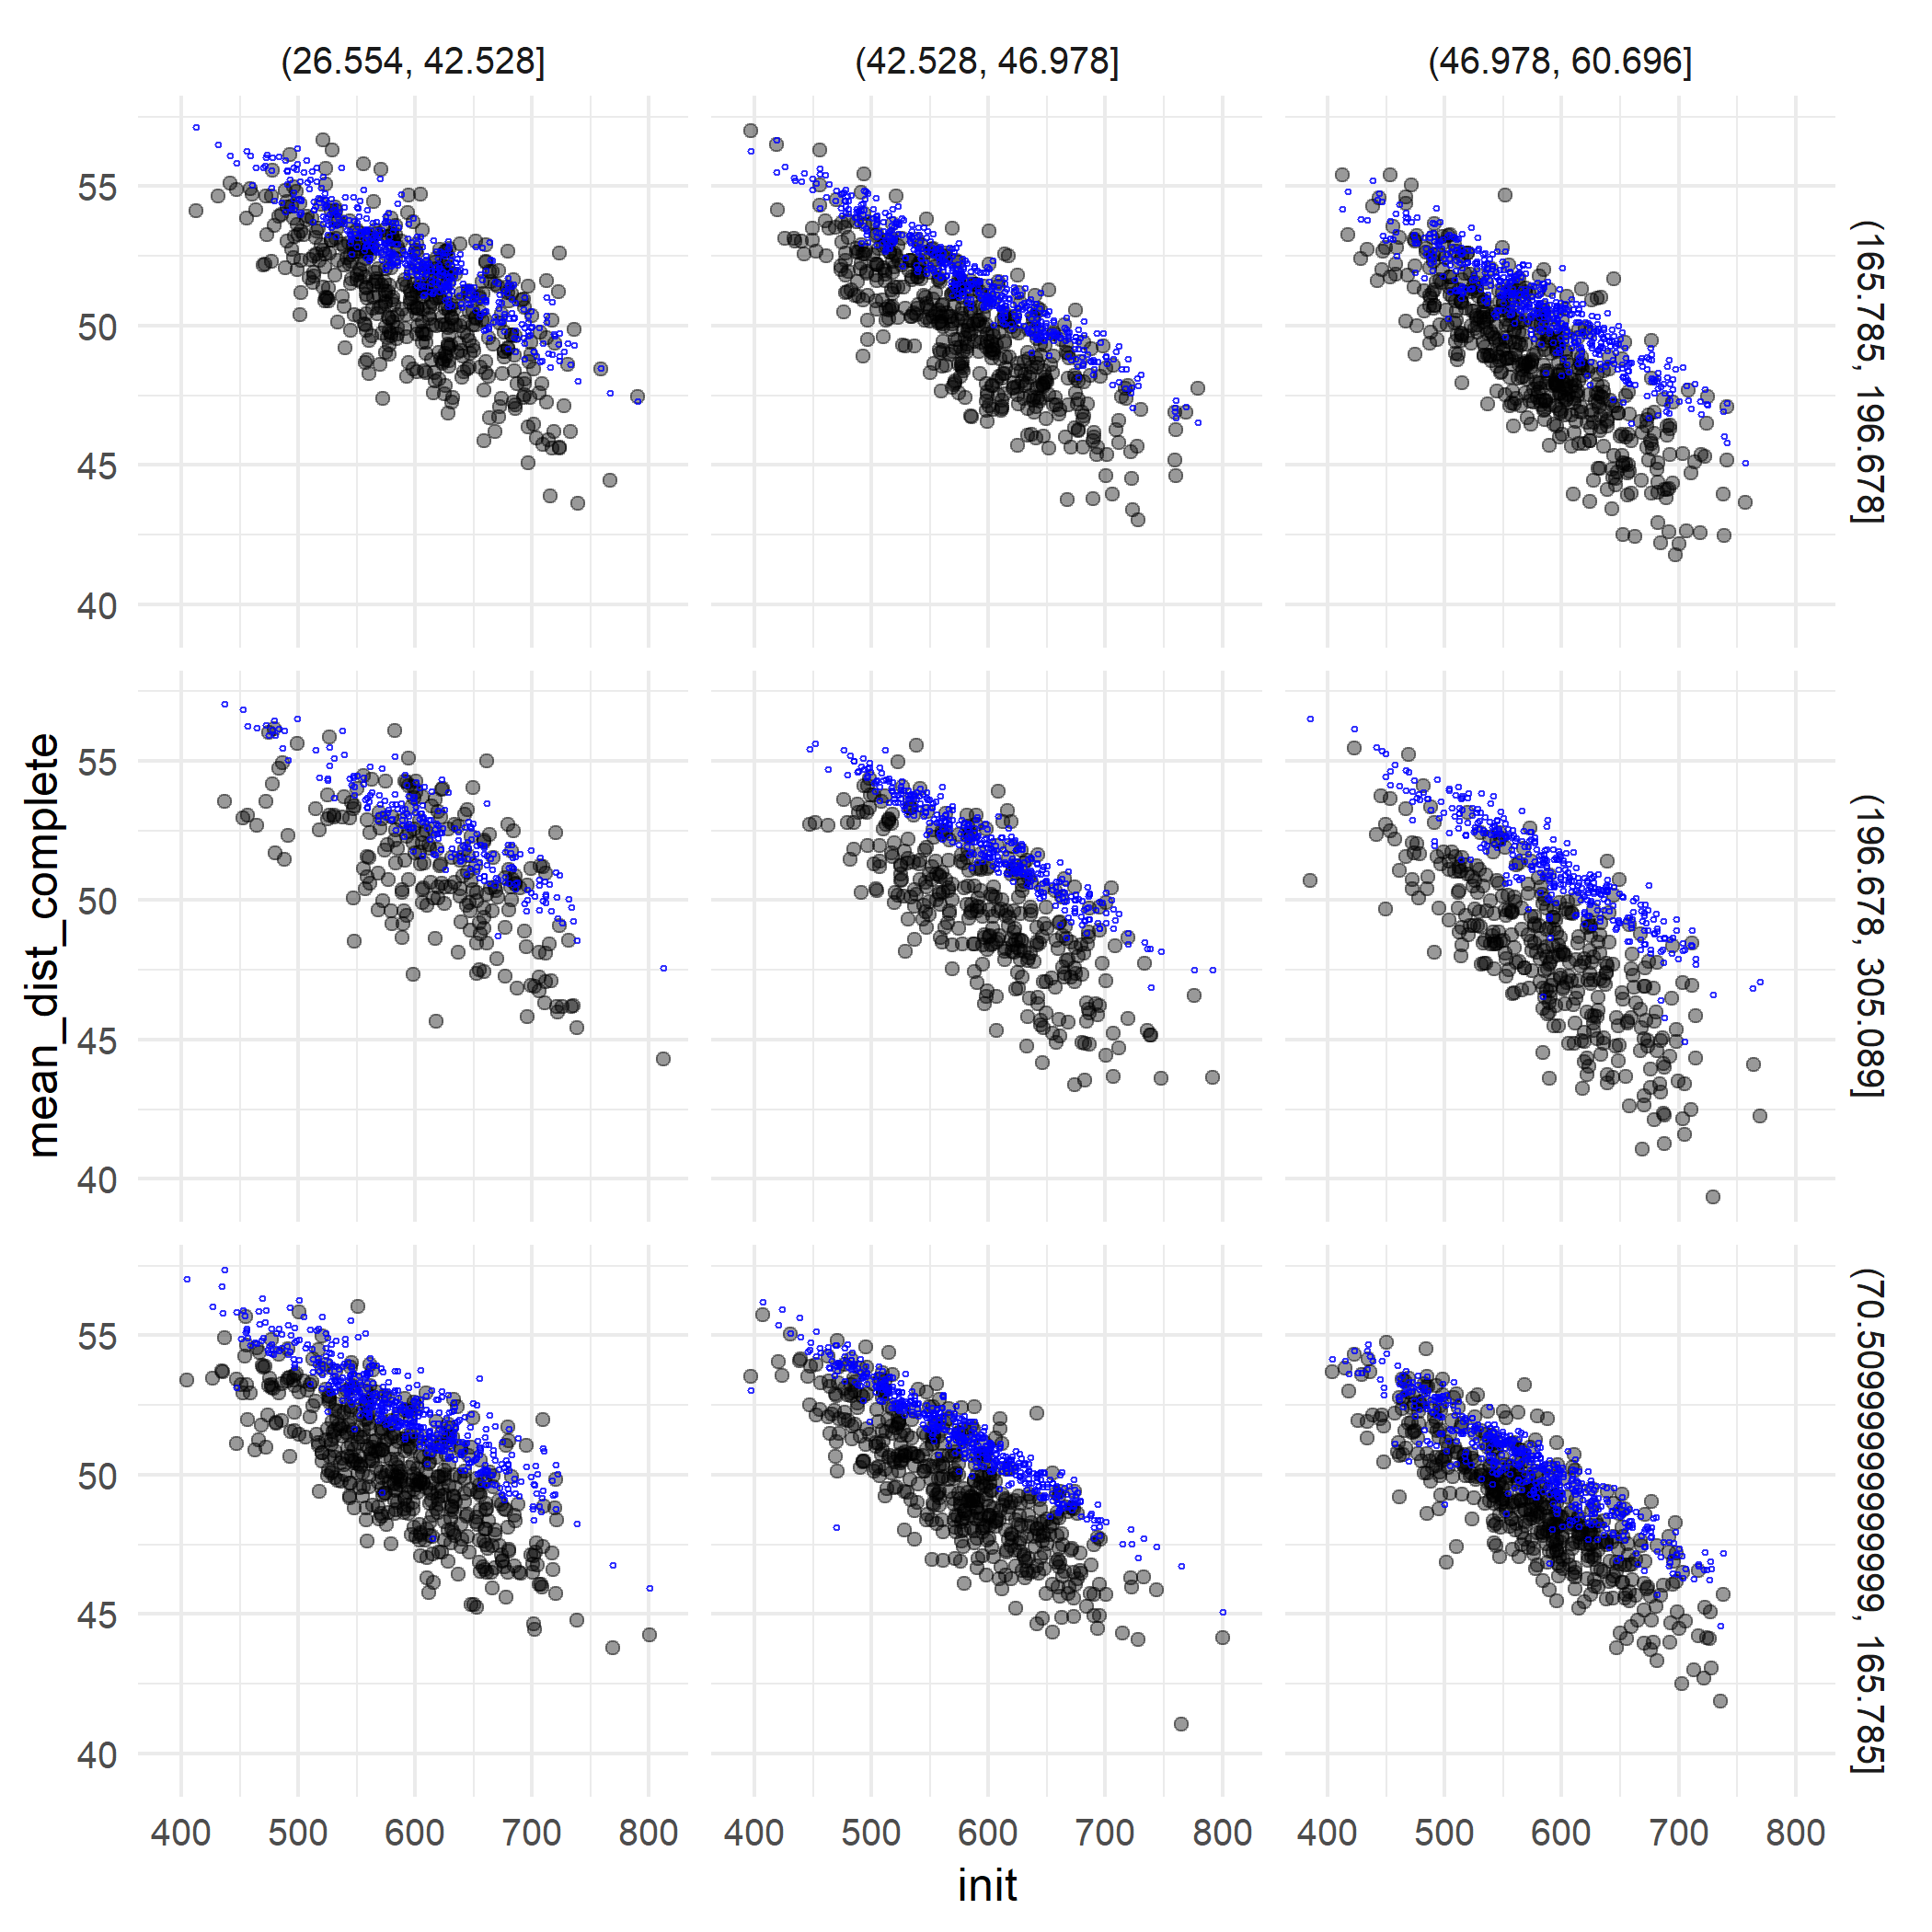
\includegraphics[width=1\linewidth]{QuantReg_mean_consum_upper_mean_dist_complete_IT000125_20190716}
{]}

\end{block}

\end{frame}

\begin{frame}

\begin{block}{Experiments}

\begin{itemize}[<+->]

\item
  Number of instances: medium (1000), large (1000) and very large
  (1000).
\item
  Time limit at 3600 seconds.
\item
  We seeded instance generation for better comparison.
\item
  CPLEX running 1 thread.
\end{itemize}

--

Largest instances have 60 aircraft, 90 periods, \textasciitilde{}30
missions (4 active missions at any given time).

\begin{enumerate}[<+->]

\item
  Create forecasting model based in 5000 small instances.
\item
  Use forecasting model to predict bounds on distance between
  maintenances: \(\hat{\mu}_{t'-t}^{lb}\), \(\hat{\mu}_{t'-t}^{ub}\).
\item
  Implement the pseudo-cut:
\end{enumerate}

\begin{align}
    & m_{ip} = 0 & p_{t'} - p_t < \hat{\mu}_{t'-t}^{lb} - tol \label{eq:dist_lb} \\
    & m_{ip} = 0  &  p_{t'} - p_t > \hat{\mu}_{t'-t}^{ub} + tol \label{eq:dist_ub}
\end{align}

\begin{enumerate}[<+->]
\setcounter{enumi}{3}

\item
  Recycling.
\end{enumerate}

\end{block}

\end{frame}

\begin{frame}

\begin{block}{How good is it (performance)}

Faster solutions, more solutions.

--

.center{[}

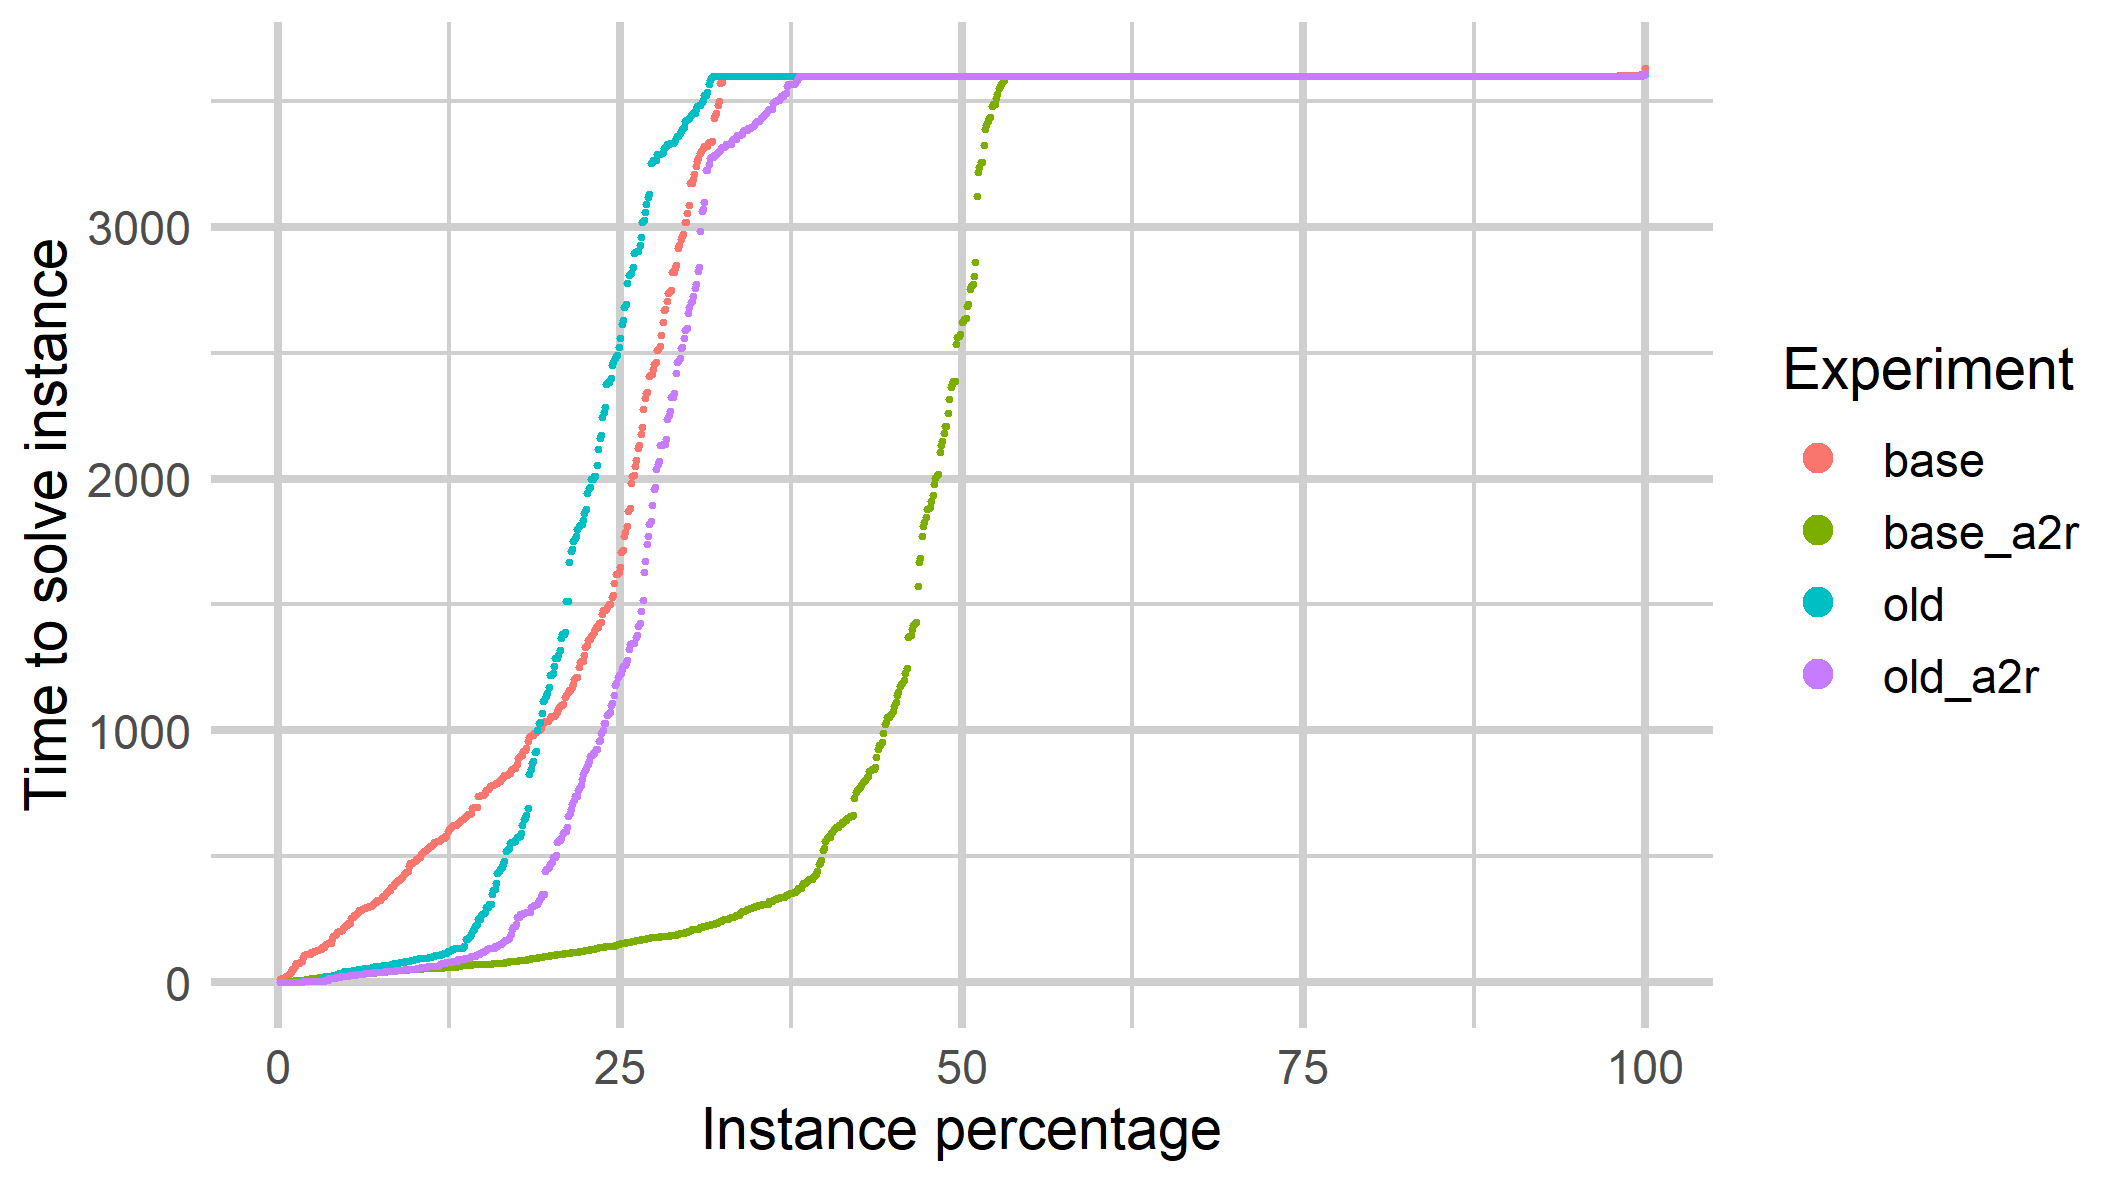
\includegraphics[width=0.8\linewidth]{time_performance_ordered_2tasks}
{]}

\end{block}

\end{frame}

\begin{frame}

\begin{block}{How good is it (optimality)}

For instances were an optimal solution was found (optimum degradation):
* 95\% of instances had less than 4\% gap with real optimal.

.center{[}

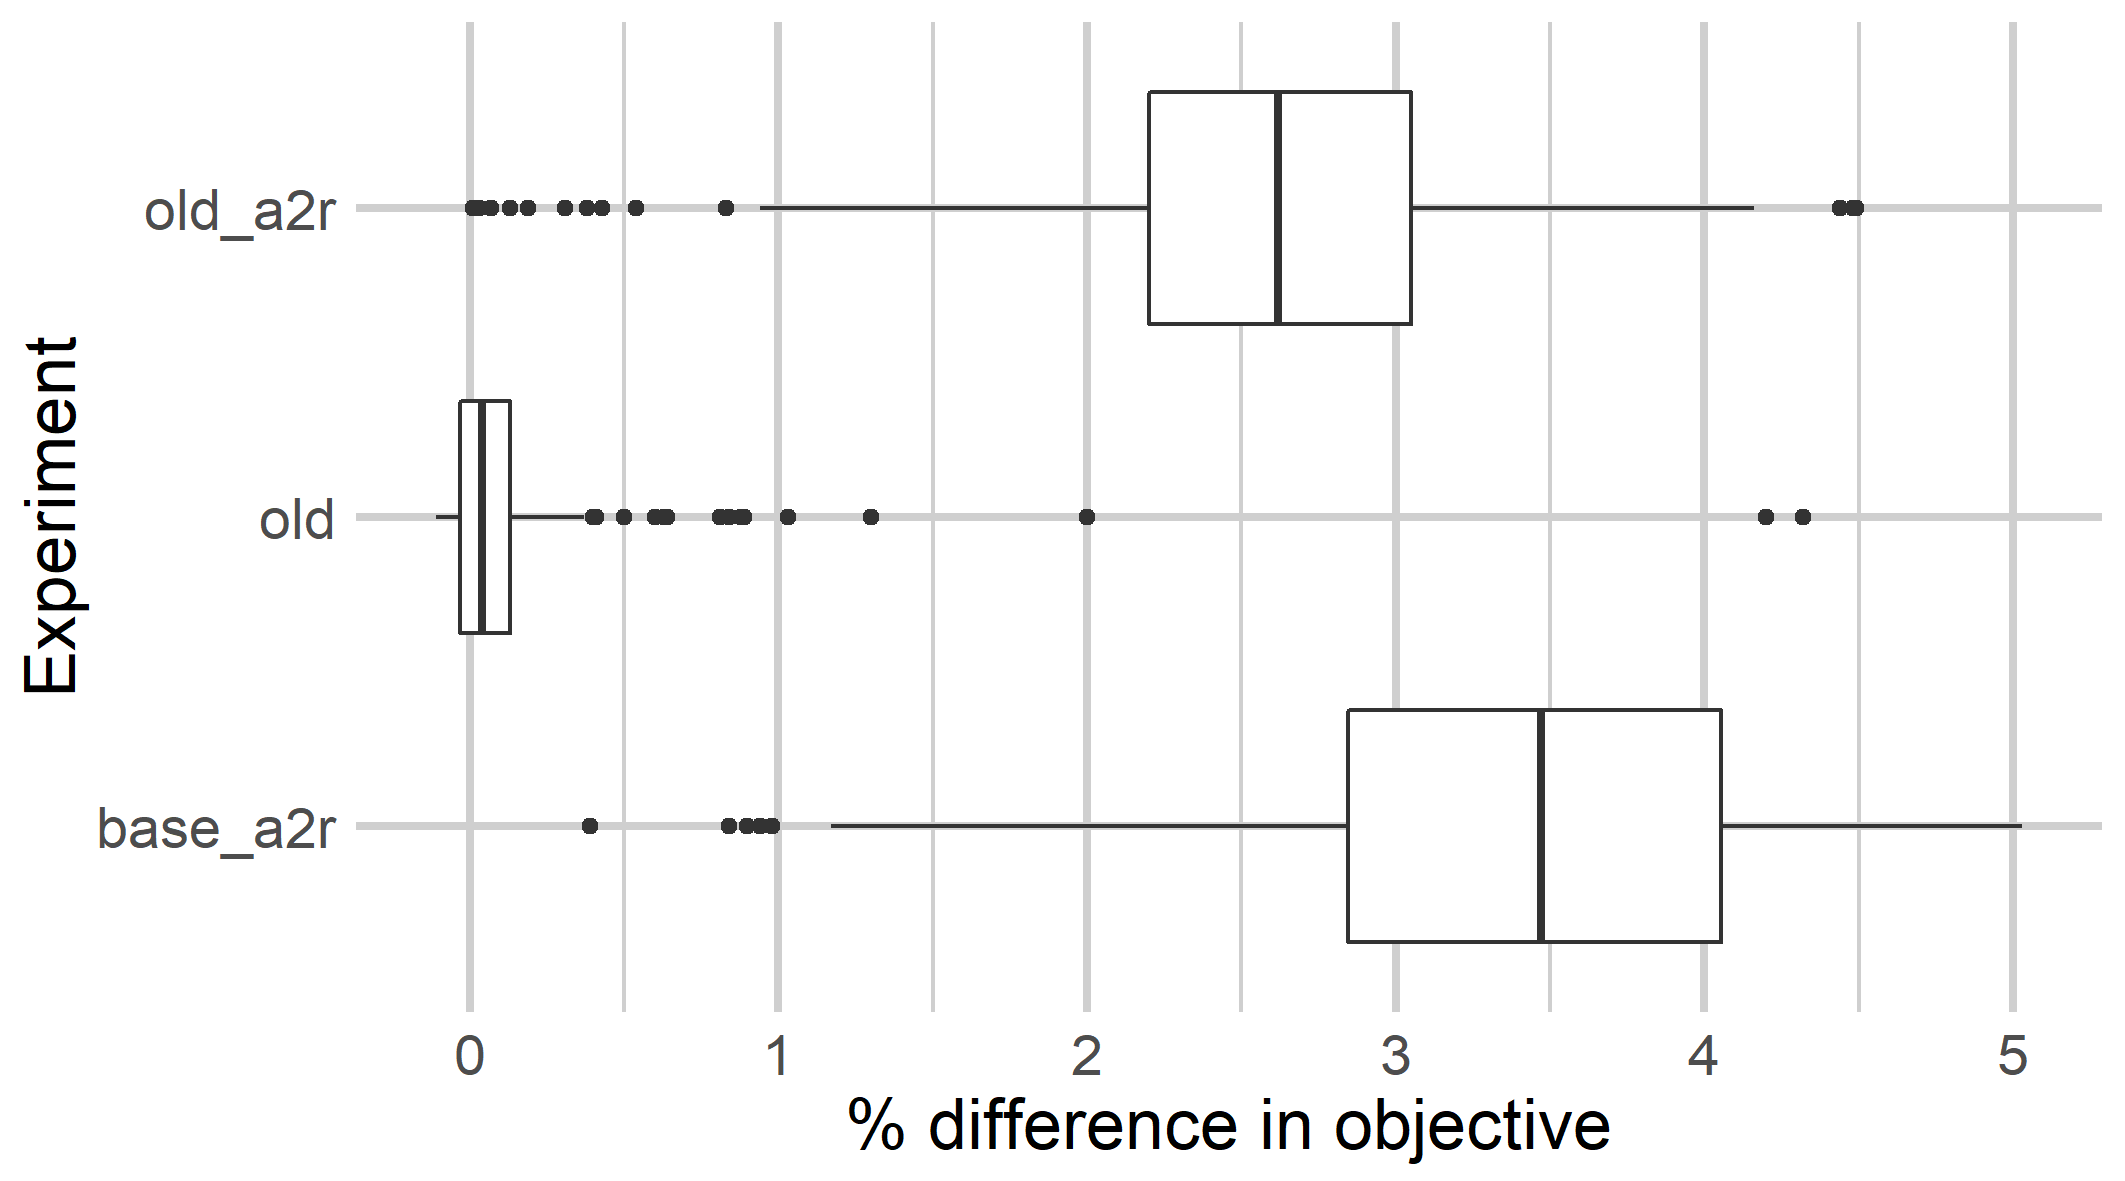
\includegraphics[width=0.8\linewidth]{quality_degradation_2tasks} {]}

\end{block}

\end{frame}

\begin{frame}{Further steps}
\protect\hypertarget{further-steps}{}

\begin{itemize}[<+->]

\item
  \textbf{Better predictions} with better features, or predicting
  several characteristics of optimal solutions.
\item
  \textbf{Predict a distribution} and sample patterns from the
  distribution instead of predicting patterns.
\item
  \textbf{Warm-start Column Generation} with a selected subset of
  potentially good patterns.
\item
  \textbf{Automatize prediction} so it can be easily integrated in other
  problems.
\end{itemize}

\end{frame}

\begin{frame}

\end{frame}

\hypertarget{references}{%
\section{References}\label{references}}

NULL

\end{document}
